\documentclass[xcolor=dvipsnames, 9pt]{beamer}
\usepackage{mathrsfs}
\usepackage{bm}
\usepackage{helvet}
\usepackage{graphicx}
\usepackage[english]{babel}
\usepackage[latin1]{inputenc}
\usepackage[absolute]{textpos}
\setlength{\TPHorizModule}{\paperwidth}
\setlength{\TPVertModule}{\paperheight}
%\usepackage{subfig}

%\setlength{\overfullrule}{2pt}
\usepackage{tikz}
\usetikzlibrary{snakes}
\usetikzlibrary{patterns}
\usetikzlibrary{arrows}

\usetheme{Frankfurt}
\useinnertheme{rounded}
\setbeamercovered{transparent}

\beamertemplatesolidbackgroundcolor{black!5}
\beamertemplatetransparentcovered

\newcommand{\greencol}{\color[RGB]{35,170,30}}
\setbeamerfont{bibfont}{size=\tiny}

\title{Design and Stabilization of a\\[0.05in]One Legged Hopper}
%\subtitle{Something catchy here}

\author[Pratik]{Pratik Chaudhari\\[0.1in]06D01015\\[0.3in]\small{Prof. Hemendra Arya\hfill Prof. Bhartendu Seth}\\[0.05in]\footnotesize{Guide\hspace{1.4in} Co-guide}}
\date{\footnotesize{B.Tech. Project}}

\AtBeginSection[]
{
    \begin{frame}<beamer>
	\frametitle{Outline}
        \small
        {
	  \tableofcontents[currentsection]
        }
	\end{frame}
}

\begin{document}
{
%\usebackgroundtemplate{\begin{textblock}{0.6}(0.3,0.55)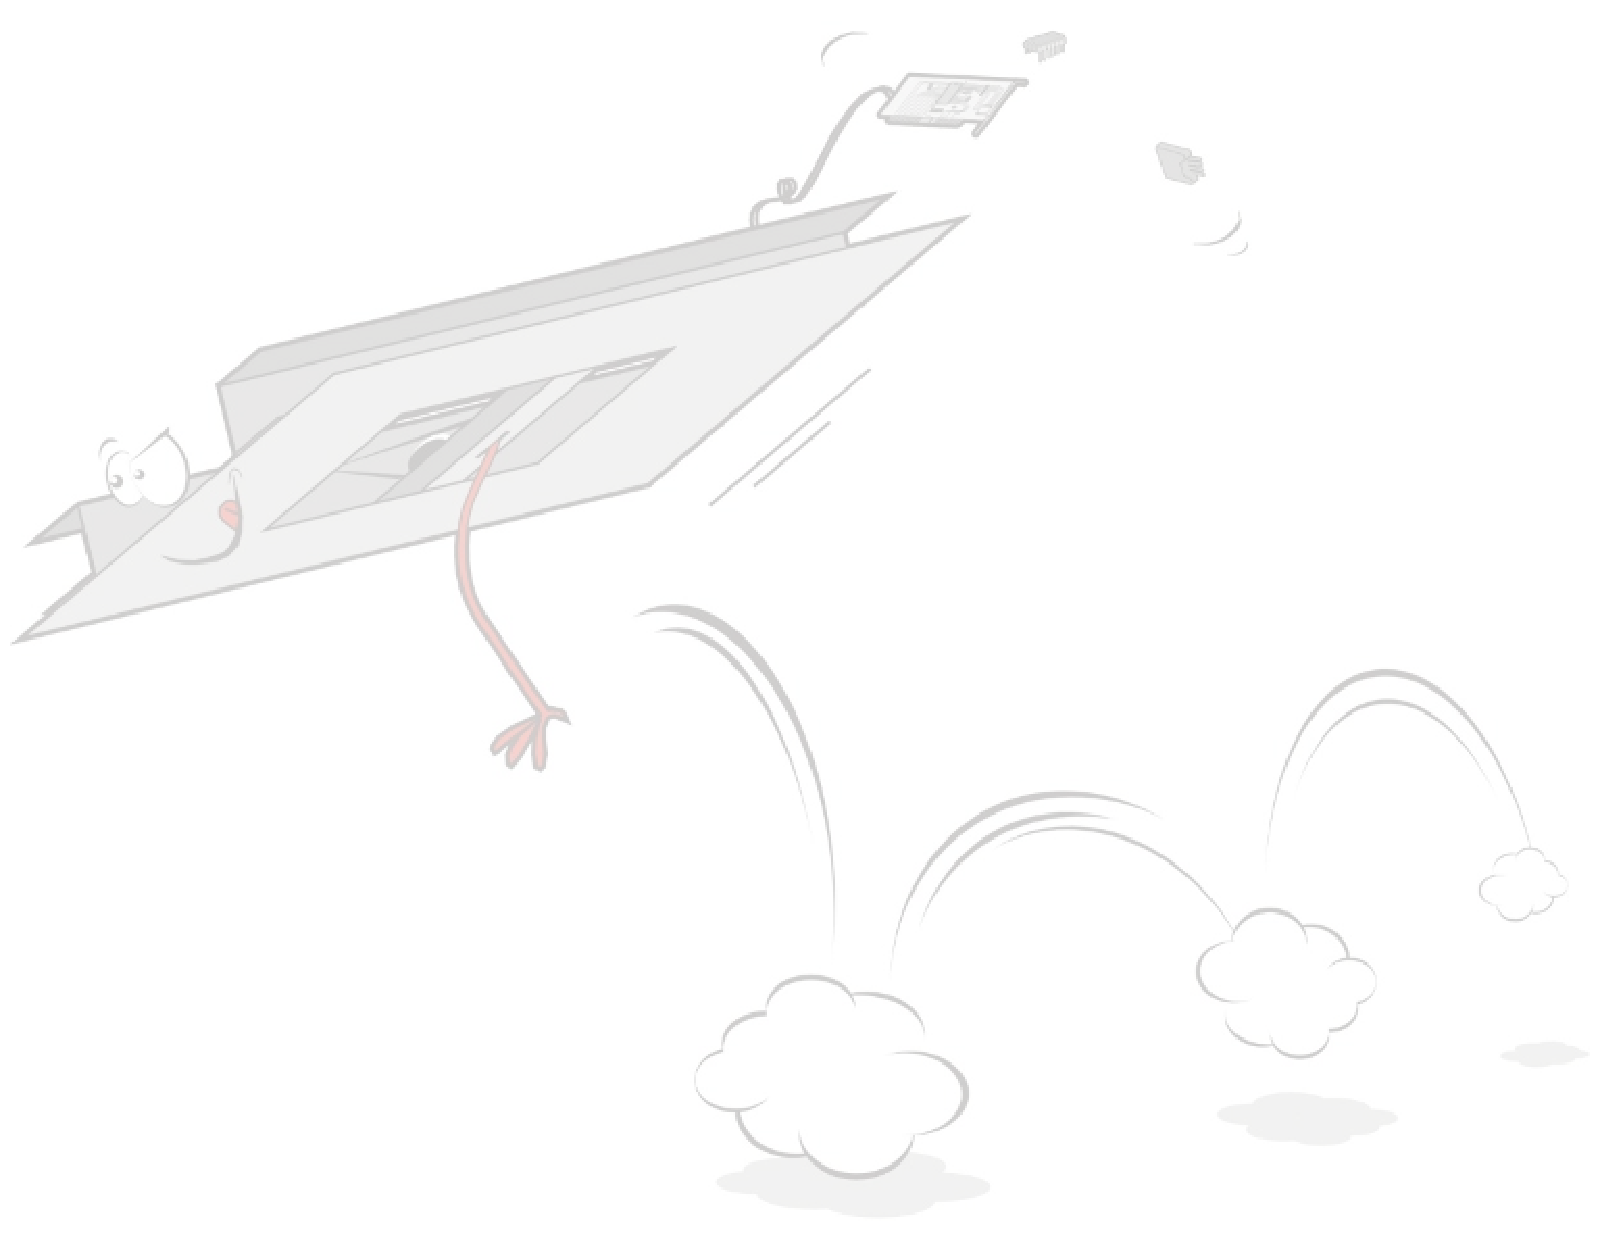
\includegraphics[scale=0.2]{fig/cartoon.pdf}\end{textblock}
\begin{frame}
\titlepage
\end{frame}
}

\section{Introduction}

\subsection*{Terminology}
\begin{frame}
\frametitle{Springy Leg Offset Mass}
\begin{columns}
\column{0.5\textwidth}
\begin{figure}
\centering
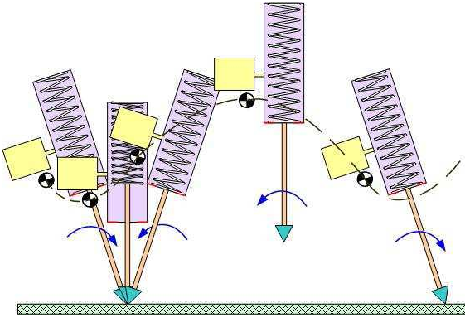
\includegraphics[width=\textwidth]{fig/SLOM_motion.pdf}
\caption{SLOM motion}
\end{figure}

\column{0.5\textwidth}
\begin{block}{Stages}
\begin{itemize}
\item
Lift-off\\[0.1in]
\item
Free fall\\[0.1in]
\item
Touch-down\\[0.1in]
\item
Stance
\end{itemize}
\end{block}
\begin{block}{Terms}
\begin{itemize}
\item
Energy Pumping Mechanism\\[0.1in]
\item
Constraint\\[0.1in]
\item
Energy Release\\[0.1in]
\end{itemize}
\end{block}

\end{columns}
\end{frame}

\subsection*{Aims}
\begin{frame}
\uncover<1->
{
\begin{block}{Design of robot}
\begin{itemize}
  \item Efficient EPM\\[0.1in]
  \item Reaction wheel\\[0.1in]
  \item Onboard electronics
\end{itemize}
\end{block}
}
\uncover<2->
{
\begin{block}{Theory}
\begin{itemize}
  \item Non-linear model\\[0.1in]
  \item Initial conditions\\[0.1in]
  \item In-place hopping\\[0.1in]
  \item Running gait
\end{itemize}
\end{block}
}
\uncover<3->
{
\begin{block}{Experiments}
\begin{itemize}
  \item Attitude estimation\\[0.1in]
  \item Fabrication and interfacing of electronics
\end{itemize}
\end{block}
}
\end{frame}


\section{Design}
\subsection*{Final Design}

\begin{frame}
\frametitle{Final Design}

\begin{columns}

\column{0.5\textwidth}
\begin{figure}
\centering
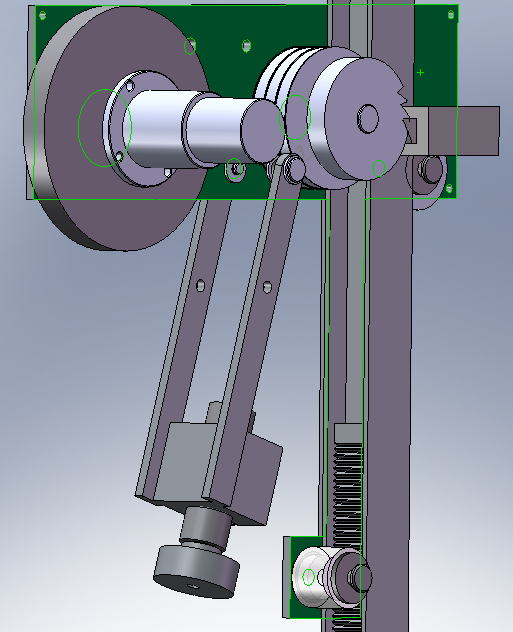
\includegraphics[width=\textwidth]{fig/hopper_detach.png}
\caption{Detached motor sleeve}
\end{figure}

\column{0.5\textwidth}
\begin{block}{Features}
\begin{itemize}
\item
{\greencol EPM :}\\[0.1in]
    \begin{itemize}
    \item
    Motor travels down on rack\\[0.1in]
    \item
    Dual springs, helical gears and slant rack\\[0.1in]
    \end{itemize}
\item
{\greencol Constraint :}\\[0.1in]
    \begin{itemize}
    \item
    Ratchet and Paul\\[0.1in]
    \item
    Band drive\\[0.1in]
    \item
    Disengage motor sleeve\\[0.1in]
    \end{itemize}
\end{itemize}
\end{block}
\end{columns}
\end{frame}

\begin{frame}
\begin{columns}
\column{0.5\textwidth}
\begin{figure}
\centering
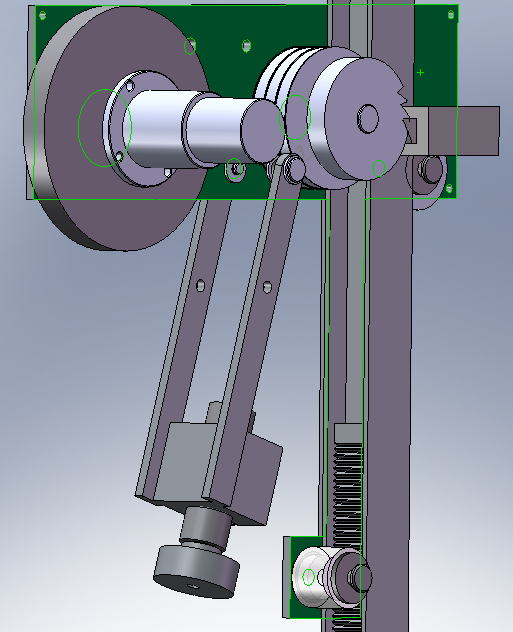
\includegraphics[width=\textwidth]{fig/hopper_detach.png}
\caption{Detached motor sleeve}
\end{figure}

\column{0.5\textwidth}
\begin{figure}
\centering
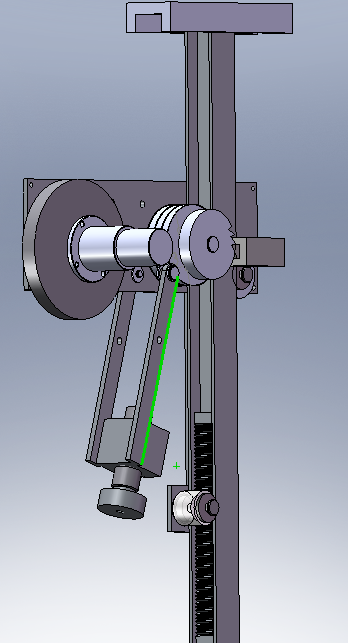
\includegraphics[scale = 0.4]{fig/hopper_bot.png}
\caption{Full Robot}
\end{figure}
\end{columns}
\end{frame}


\begin{frame}
\frametitle{Final Design}
\begin{columns}

\column{0.5\textwidth}
\begin{figure}
\centering
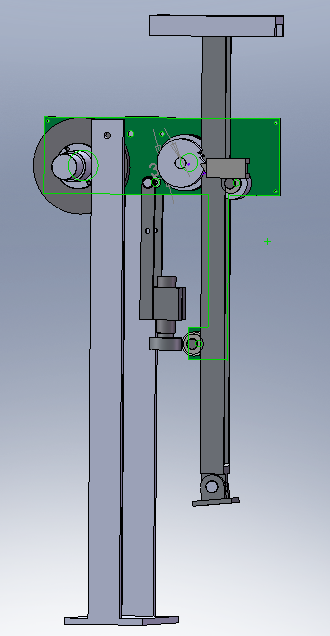
\includegraphics[scale=0.4]{fig/hopper_iso.png}
\caption{Test Rig}
\end{figure}

\column{0.5\textwidth}
\begin{block}{Features}
\begin{itemize}
\item
{\greencol Test-rig :}\\[0.1in]
    \begin{itemize}
    \item
    Pivoted near the C.G.\\[0.1in]
    \item
    Attitude re--orientation\\[0.1in]
    \item
    Simulated hopping\\[0.1in]
    \end{itemize}
\item
{\greencol Overall :}\\[0.1in]
    \begin{itemize}
    \item
    Height : $\sim$ 500 mm\\[0.1in]
    \item
    Leg $\sim$ 0.7 kg\\[0.1in]
    \item
    Total $\sim$ 4.7 kg\\[0.1in]
    \item
    Disengage motor sleeve\\[0.1in]
    \end{itemize}
\end{itemize}
\end{block}
\end{columns}
\end{frame}
\section{Modeling}

\subsection*{Equations}

\begin{frame}
\frametitle{Equations of motion}

\begin{block}{Euler--Lagrangian equations}
\begin{equation*}
 T =\frac{1}{2}\left[m_w(\dot{x_w}^2 + \dot{y_w}^2) + m_p (\dot{x_p}^2 + \dot{y_p}^2)
  + m_l(\dot{x_l}^2 + \dot{y_l}^2) +  J_w(\dot{\phi} + \dot{\theta})^2
  + J_b\dot{\theta}^2\;\right]
\end{equation*}
\vspace{2mm}
\begin{equation*}
V\:=\: g\:\left[\: m_l\:y_l\:+\: m_w\:y_w\:+\: m_p\:y_p\:\right] + \frac{1}{2}K\:(l - l_0)^2
\end{equation*}
\vspace{2mm}
\begin{equation*}
L = T - V
\end{equation*}
\vspace{2mm}
\begin{equation*}
q = \left[\:x\;\;\;y\;\;\;l\;\;\;\theta\;\;\;\phi\:\right] 
\end{equation*}
\vspace{2mm}
\begin{equation*}
\frac{d}{dt}\left(\frac{\partial\:L}{\partial\:\dot{q_A}}\right) - \frac{\partial\:L}{\partial\:q_A} = Q_A
\end{equation*}
\vspace{2mm}
\begin{equation*}
 Q_A = \sum_{r=1}^m\lambda_r\;\frac{\partial \psi_r}{\partial q_A}
\end{equation*}

\end{block}
\end{frame}

\begin{frame}
\frametitle{Stance Phase}
\begin{block}{Stance Phase}
\begin{itemize}
 \item
  Foot touches the ground when,
  \begin{equation*}
  y(t) = (\;l_{impact} - l_0\;)\:\cos \theta_{impact} + d \sin \theta_{impact}
  \end{equation*}\\[0.1in]
  \item
  Constraint equations,
  \begin{eqnarray*}
    y(t) = (\;l(t) - l_0\;)\:\cos \theta + d \sin \theta\\
    x(t) = x_{f-impact} - (\;l(t) - l_0\;)\:\sin \theta - d \cos \theta
  \end{eqnarray*}
  where
  \begin{equation*}
  x_{f-impact} =  x_{impact} + (\;l_{impact} - l_0\;)\:\sin \theta_{impact} + d \cos \theta_{impact}
  \end{equation*}
  \item
  Phase ends when
  \begin{equation*}
  l(t) = l_0 
  \end{equation*}

  \end{itemize}

\end{block}

\end{frame}


\begin{frame}
\frametitle{Flight Phase}
\begin{block}{Spring Controller}
\begin{itemize}
  \item
  \begin{equation*}
  \ddot{l}(t) = \left\{\begin{array}{ll}
			0 & l(t) \leq (l_0 - \epsilon)\;\;OR\;\;l(t) \geq (l_{max} + \epsilon)\\
			&\\
			l_{accel} & l_0 \leq l(t) \leq \frac{(l_{max} + l_0)}{2}\\
			&\\
			-l_{accel} & \frac{(l_{max} + l_0)}{2} \leq l(t) \leq l_{max}
                      \end{array} \right.
  \label{eqn:4_spring_retract}
  \end{equation*}\\[0.1in]
    \item
    Convert $\ddot{l}(t)$ control law to implementable $\dot{l}(t)$ form\\[0.1in]
   \item 
    Sense $\omega(t)$ with encoders,
    \begin{equation*}
    e(t) = \omega(t) - \omega_d(t)
    \end{equation*}\\[0.1in]
    \begin{equation*}
    U_{l}(t) = K_w\;\omega_d(t) + K_p\;e(t) + K_d\;\frac{d\;e(t)}{dt} + K_i\;\int e(t)\;dt
    \label{eqn:4_l_controller}
    \end{equation*}

\end{itemize}
\end{block}
\end{frame}

\begin{frame}
\frametitle{Spring Phase}
\begin{block}{Constrainted flight phase}
\begin{itemize}
  \item
  Constraint is,
  \begin{equation*}
  l(t) = l_{max}
  \end{equation*}
  \item
  Solver stops when,
  \begin{equation*}
  y(t) = (\;l(t) - l_0\;)\:\cos \theta + d \sin \theta
  \end{equation*}

\end{itemize}
\end{block}
\vspace{0.1in}
\begin{figure}
\centering
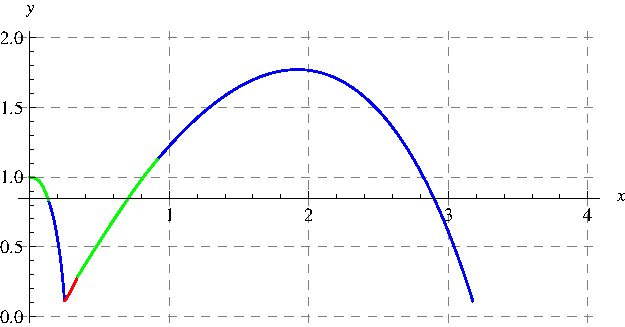
\includegraphics[width=0.7\textwidth]{fig/plotG.pdf}
\caption{Equations of motion propagation}
\end{figure}
\end{frame}

\subsection*{Initial Conditions}
\begin{frame}
\frametitle{Initial Conditions}
\begin{itemize}
  \item 
  Topmost point of the trajectory,\\ i.e. $x = 0$, $\dot{x} = 1$, $\dot{y} = 0$, $y = 1$, $\phi$ is constrained\\[0.1in]
  \item
  Calculate the amount of energy lost in the impact to give $l_{max} = 0.37 m$\\[0.1in]
  \item
  Vary $\theta_0$ and $\dot{\theta}_0$ to minimize norm\\[0.1in]
  \item
  Define norm as,
  \begin{equation*}
  norm = \sum_{i = 1, i\;\neq\;1, 5, 10}^{10} || q_{A_i} - q_{B_i} ||
  \end{equation*}\\[0.1in]
  Remove $x(t)$, $\phi(t)$ and $\dot{\phi}(t)$ from the norm\\[0.1in]
  \item
  Problems with optimizing algorithm, hence manual search\\[0.1in]
  \item
  $\theta_0 = 0$ and $\dot{\theta}_0 = -0.5$ rad/s
\end{itemize}
\end{frame}

% \begin{frame}
% \frametitle{Poincare Map}
% \begin{block}{Linear Poincare Map}
% \begin{itemize}
%   \item 
%   
% \end{itemize}
% 
% \end{block}
% 
% \end{frame}


\section{Gaits}
\subsection*{Inplace hopping}
\begin{frame}
\frametitle{In-place hopping}
\begin{block}{Controller}
\begin{itemize}
  \item 
  Impact torque destabilizing, control robot attitude\\[0.1in]
  \item
  Flight, spring phases : $\theta_d = 0$\\[0.1in]
  \item
  Stance phase,
  \begin{equation*}
   \theta_d = \tan^{-1}\left(\frac{x_{impact}}{h_{max}}\right)
  \end{equation*}\\[0.1in]
\end{itemize}
  
  \begin{columns}
  \column{0.5\textwidth} 
  \begin{figure}
  \centering
  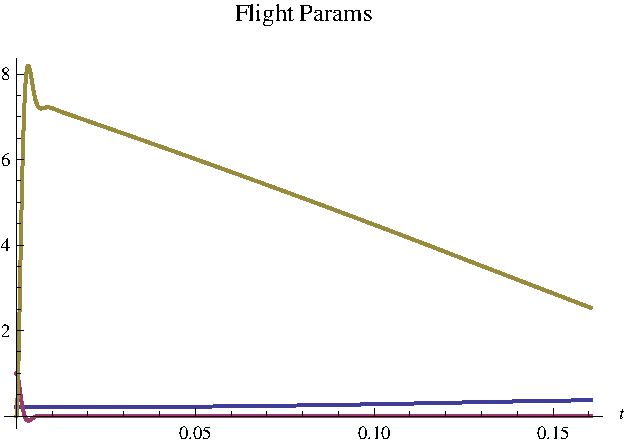
\includegraphics[scale=0.45]{fig/inplace_pFlight_params.pdf}
  \end{figure}
  
  \column{0.5\textwidth} 
  \begin{figure}
  \centering
  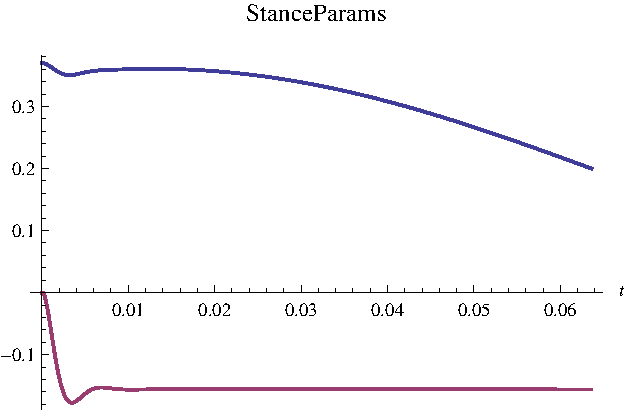
\includegraphics[scale=0.45]{fig/inplace_pStance_params.pdf}
  \end{figure}
  \end{columns}
  \begin{itemize}
    {
    \small
    \item 
    $l(t)$ - Blue, $\theta(t)$ - Pink, $\phi(t)$ - Yellow, t = secs
    }
  \end{itemize}

\end{block}

\end{frame}

\begin{frame}
\frametitle{Inplace : Trajectory}
\begin{itemize}
 \item
  Start at $y = 1$m, $\theta = 1$ rad, $\dot{\theta} = -1$ rad/s
\end{itemize}
  \begin{figure}
  \centering
  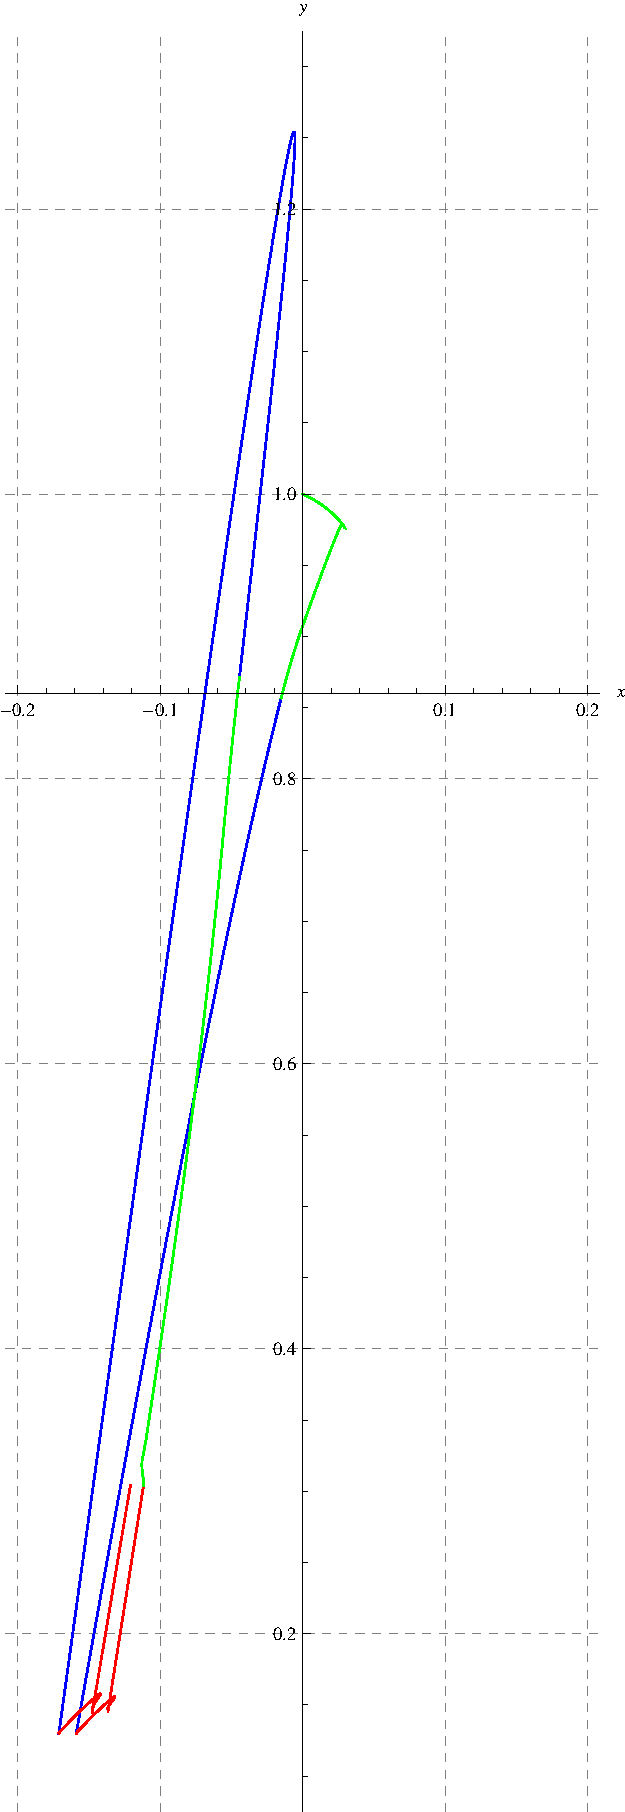
\includegraphics[scale=0.2]{fig/plot_inplace.pdf}
  \caption{Inplace : Trajectory}
  \end{figure} 
\end{frame}

\subsection*{Running}
\begin{frame}
\frametitle{Stance controller}
\begin{block}{Details}
\begin{itemize}
  \item
  Most important phase for control\\[0.1in]
  \item
  Generate $\theta_G(t)$ using good initial conditions\\[0.1in]
  \item
  PID torque controller for $e = \theta - \theta_G$\\[0.1in]
\end{itemize}
  \begin{figure}
  \centering
  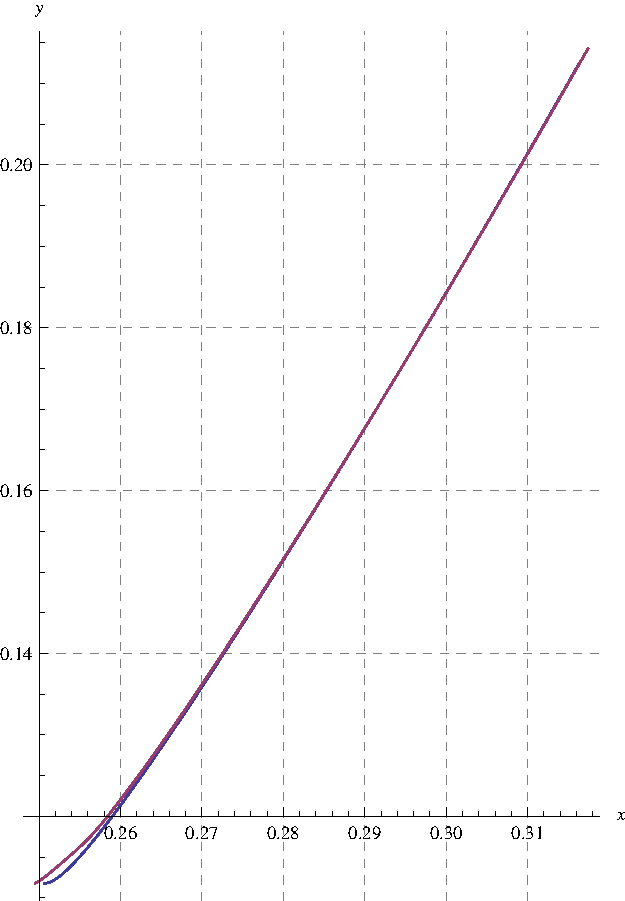
\includegraphics[scale=0.4, angle = 270]{fig/pStance_trajec_control.pdf}
  \caption{Good - Blue, Perturbed - Pink, distances in meters}
  \label{fig:stance_control_trajec}
  \end{figure}

\end{block}
\end{frame}

\begin{frame}
\frametitle{Flight, Spring phases}
\begin{block}{Control}
\begin{itemize}
  \item
  Large time--scales\\[0.1in]
  \item
  Solve attitude reorientation to impact attitude\\[0.1in]
\end{itemize}
  \begin{equation*}
     \Delta\;\theta (t)= \theta_{impact} - \theta(t)
    \end{equation*}\\[0.1in]
    \begin{equation*}
    \ddot{\phi}_d(t) = \left(\frac{-2\;J_b}{J_w}\right) \left(\frac{\Delta\;\theta - \dot{\theta}(t)\;t_{left}}{t_{left}^2}\right)
    \end{equation*}\\[0.1in]

    \begin{equation*}
     e(t) = \ddot{\phi}(t) - \ddot{\phi}_d(t)
    \end{equation*}
    \begin{equation*}
     U_{\phi}(t) = \ddot{\phi}_d(t) + K_p\;e(t) + K_d\;\dddot{\phi}(t) + K_i\;\;\int \phi dt
    \end{equation*}
\end{block}
\end{frame}

\begin{frame}
  \frametitle{Controlled trajectory}
  \begin{itemize}
    \item
    Perturb attitude at liftoff
  \end{itemize}

  \begin{figure}
  \centering
  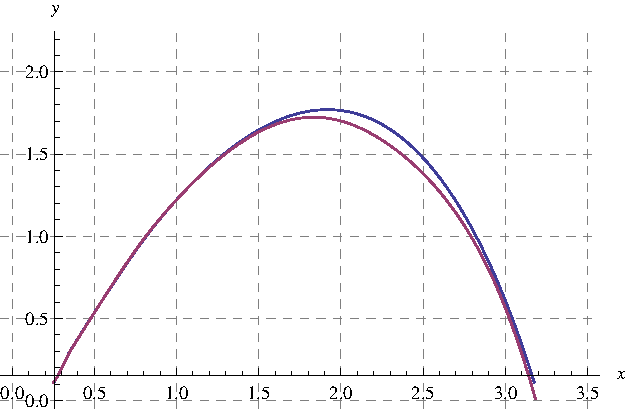
\includegraphics[scale=0.8]{fig/pFullTrajec_control.pdf}
  \caption{Trajectory Controller : Good - Blue, Perturbed - Pink}
  \label{fig:full_trajec_control}
  \end{figure}

\end{frame}

\section{Attitude Estimation}

\subsection*{Hardware}
\begin{frame}
\frametitle{ReWac Board Hardware}
    \begin{columns}
        \column{0.6\textwidth}
        \begin{figure}
        \centering
        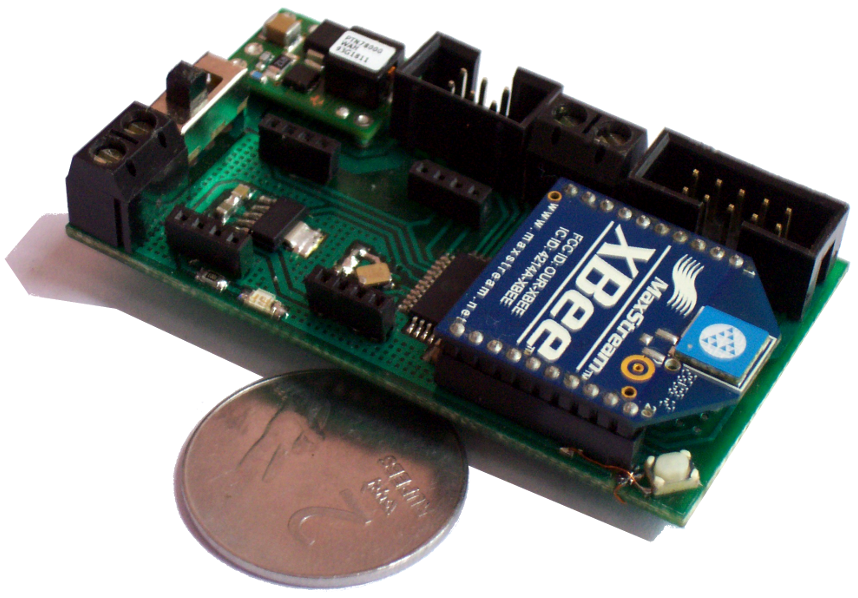
\includegraphics[scale=0.2]{fig/rewac.png}
        \end{figure}
        
        \column{0.4\textwidth}
        \begin{itemize}
        \item
        Microchip dsPIC33F\\[0.05in]
        16 bit, 40 MIPS\\[0.1in]
        \item
        Accelerometer\\[0.05in]
        2.162 LSB/mg\\[0.1in]
        \item
        Gyroscope (50 Hz)\\[0.05in]
        0.07326 $^o/s/$LSB\\[0.1in]
        \item
        Self-made MOSFET motor driver\\[0.1in]
        \item
        XBee module\\[0.1in]
        \end{itemize}
    \end{columns}
\end{frame}

\begin{frame}
\frametitle{Kalman Filter}
\begin{block}{Why}
\begin{itemize}
\item
Pitch attitude estimate
\item
Computing power
\end{itemize}
\end{block}

\begin{block}{How}
\begin{equation*}
\bm{x} = [x_1\;\;x_2]^T = [\theta\;\;\dot{\theta}]^T
\end{equation*}
\vspace{0.075in}
\begin{equation*}
\bm{x}_{k+1} = \bm{A}\:\bm{x}_k + \bm{B}\:\bm{u}_k + \bm{w}_k
\end{equation*}
\vspace{0.075in}
\begin{equation*}
y_{k+1} = \bm{C}\:\bm{x}_{k+1} + z_{k+1}
\end{equation*}
\end{block}

\begin{block}{Tricks}
\begin{itemize}
\item
\alert{Sparse covariance matrix}
\item
Remove matrix operations
\item
\alert{Fixed point arithmetic}
\end{itemize}
\end{block}
\end{frame}

\begin{frame}
\frametitle{High Frequency Input sampled at 50 Hz}
\begin{figure}
\centering
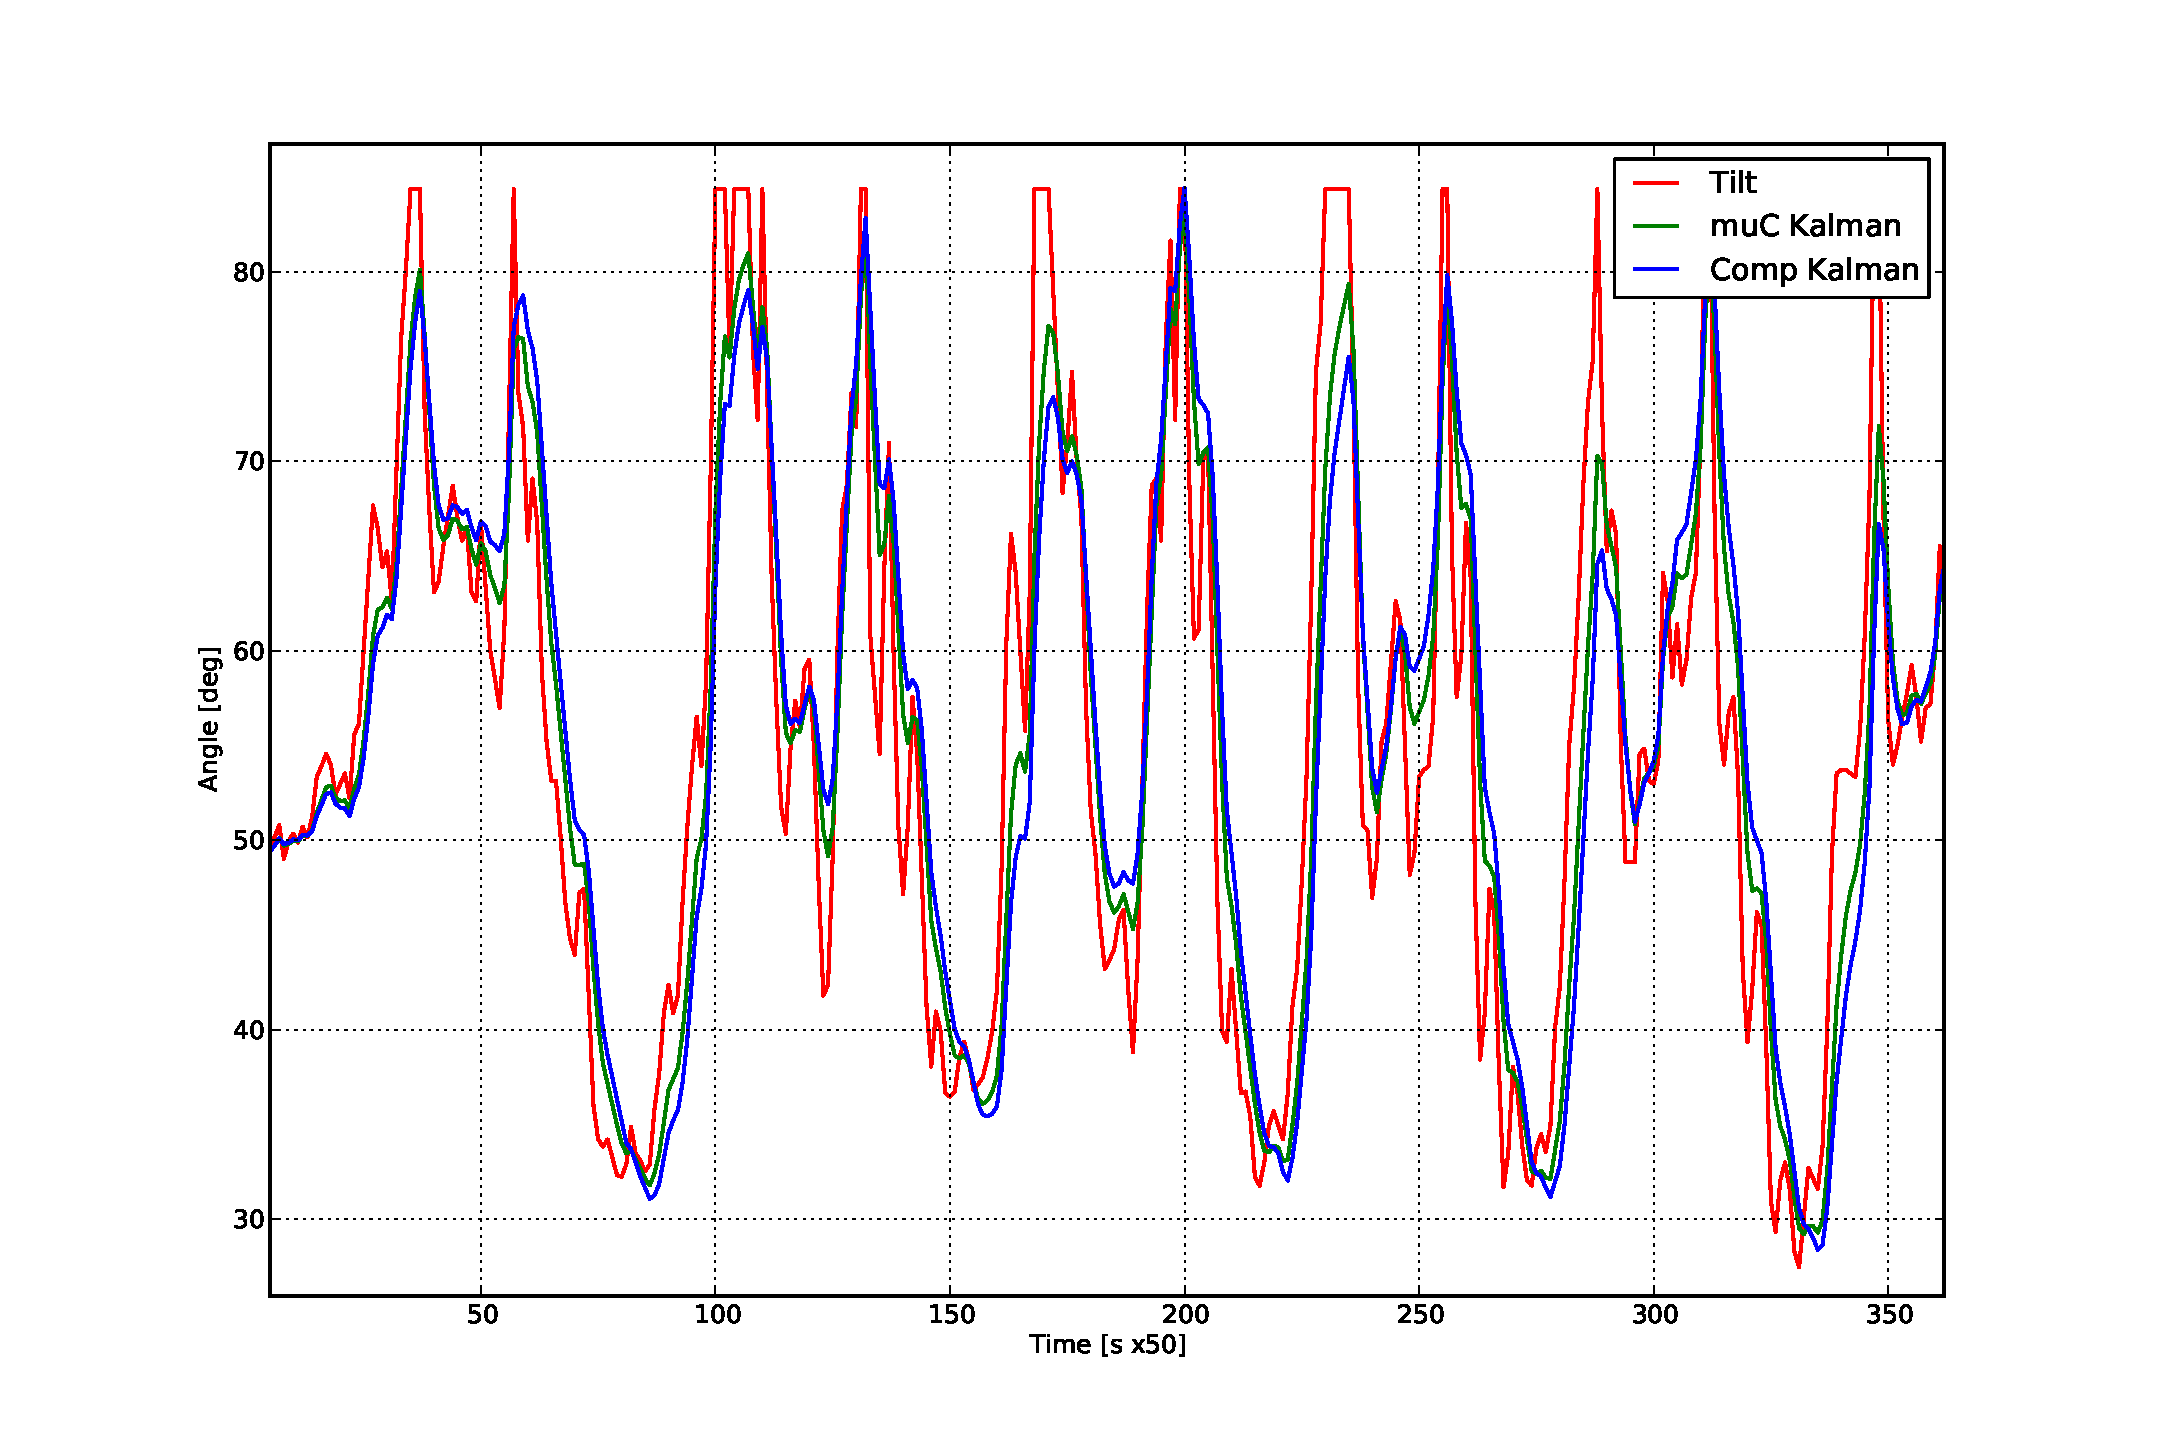
\includegraphics[width=\textwidth]{fig/kf_fp_hf.pdf}
\end{figure}
\end{frame}
\section{Conclusion}

\begin{frame}
\frametitle{Summary}
\begin{block}{Fabrication}
\begin{itemize}
  \item 
  Robot fabrication almost done\\[0.1in]
  \item
  Electronics ready\\[0.1in]
\end{itemize} 
\end{block}\\[0.2in]

\begin{block}{Controller}
\begin{itemize}
  \item 
  In-place hopping solved\\[0.1in]
  \item
  More work on trajectory following\\[0.1in]
\end{itemize} 
\end{block}\\[0.2in]

\begin{block}{Future Work}
\begin{itemize}
  \item 
  Assisted test-rig control\\[0.1in]
  \item
  Running on treadmill
\end{itemize} 
\end{block}
\end{frame}


\end{document}


